\documentclass{article} % For LaTeX2e
\usepackage{naaclhlt2016}
\usepackage{times}
\usepackage{latexsym}
\usepackage{hyperref}
\usepackage{url}
\usepackage{amsmath,amsthm,amsfonts}
\usepackage{multirow}
\usepackage{xspace}
\usepackage{tikz}
\usetikzlibrary{shapes,backgrounds,patterns}
\usepackage{graphicx}
\graphicspath{ {images/} }


\newcommand{\Prob}{\mathbb{P}}
\newcommand{\todo}[1]{{\bf [[}\textcolor{blue}{ todo: #1}{\bf ]]}}
\newcommand{\fix}{\marginpar{FIX}}
\newcommand{\new}{\marginpar{NEW}}

% named as such because `\arg1' apparently isn't valid
\newcommand{\argOne}{\emph{arg1}\xspace}
\newcommand{\argTwo}{\emph{arg2}\xspace}

\newcommand{\citep}[1]{\cite{#1}}
\newcommand{\citet}[1]{\newcite{#1}}



\title{Universal Schema Without Entity Embeddings}

\author{Patrick Verga \& Andrew McCallum \\
    College of Information and Computer Sciences\\
    University of Massachusetts Amherst\\
    % Amherst, MA 01002, USA \\
    \texttt{\{pat, mccallum\}@cs.umass.edu} \\
}

\begin{document}


\maketitle

\begin{abstract}
Universal schema jointly embeds knowledge bases and textual patterns to reason about entities and relations for automatic knowledge base construction and information extraction.
In the past, entity pairs and relations were represented as learned vectors whose compatibility was determined by a scoring function.
However, this leads to cold-start problems where the model is unable to reason about entity pairs and text patterns unseen at train time.
Recently, compositional Universal Schema was proposed to address generalization to unseen text patterns.
In this work we take the next step of removing explicit entity pair representations.
Instead of learning vector representations for each entity pair in our training set, we treat an entity pair as a function of its relation.
In this paper, we experiment with several aggregation functions and demonstrate that we can perform inference using only learned relation representations.
\end{abstract}



% intro + background

\section{Introduction\label{introduction}}


\subsection {Universal Schema}
The goal of automatic knowledge base construction (AKBC) is to build a structured knowledge base (KB) of facts using a noisy corpus of raw text evidence, and perhaps an initial seed KB to be augmented~\citep{NELL,yago,freebase}. AKBC supports downstream reasoning at a high level about extracted entities and their relations, and thus has broad-reaching applications to a variety of domains.
An effective approach to AKBC is Universal Schema.
Universal Schema embeds textual patters and knowledge bases into a shared space in order to reason over relations and entity pairs.
A low dimensional embedding is learned for each entity pair and each relation type using matrix factorization.
The model is then able to infer relations between entities as the dot product between the two entity pair and relation type vectors.

Unfortunately, this formulation limits the generalization of the model.
In its original form, Universal Schema can only reason about entity pairs and textual relations explicitly seen at training time.

\subsection {Compositional Universal Schema}

Recently Universal Schema has been extended to deal with compositional representations of textual relations \citep{toutanova2015representing,verga2015multilingual}
Compositional Universal Schema has two main advantages over explicit modeling of textual patterns.
The first is tt allows for the model to share statistics between very similar patterns.
Instead of modeling the text pattern 'lives in the city' and 'lives in the city of' as distinct atomic units, they can instead be composed compositionally of the same word embeddings.
Second, and even more importantly, Compositional Universal Schema allows us to generalize to all possible textual patterns, allowing us to reason over any arbitrary text.

\begin{figure}[h]
\caption{Top : Universal Schema expresses each textual pattern as an atomic unit \protect\citet{riedel2010modeling}.
Bottom : Compositional Universal Schema uses an lstm to encode each textual relation \protect\cite{verga2015multilingual}. }
\centering
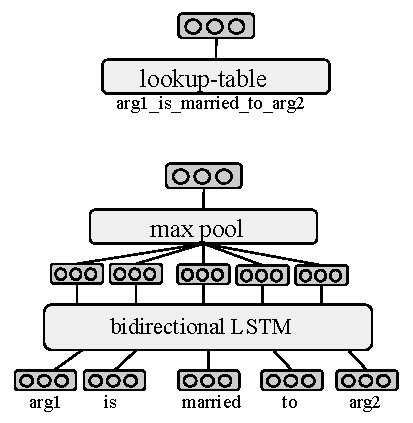
\includegraphics[scale=.68]{relation-models}
\end{figure}

\subsection {Universal Schema without Entity Embeddings}

While Compositional Universal Schema addresses reasoning over arbitrary textual patterns, it is still limited to reasoning over entity pairs seen at training time.
\citet{verga2015multilingual} approach this problem by using Universal Schema as a sentence classifier - directly comparing a textual relation to a kb relation to perform relation extraction.
However, this approach is unsatisfactory for two reasons.
The first is that this creates an inconsistency between training and testing, as the model is trained to predict compatibality between entity pairs and relations and not relations directly.
Secondly, it considers only a single piece of evidence while making its prediction.

The learned entity pair can be seen as a sumamrization of all relations for which that entity pair was seen.


Rather than modeling each entity pair as an explicit vector, we instead treat each entity pair as an aggregate function over each of its relation types.
This allows us to trivially extend to unseen entity pairs, have a direct link to provenance, and allocate a variable number of parameters per entity pair.


\subsection {Entities vs Entity Pairs}

A knowledge base is naturally described as a graph, in which entities are nodes and relations are labeled edges~\citep{yago,freebase}.
In the case of \emph{knowledge graph completion}, the task is akin to link prediction, assuming an initial set of (\emph{s, r, o}) triples.
See~\citet{nickel2015review} for a review.
No accompanying text data is necessary, since links can be predicted using properties of the graph, such as transitivity.
In order to generalize well, prediction is often posed as low-rank matrix or tensor factorization.
A variety of model variants have been suggested, where the probability of a given edge existing depends on a multi-linear form~\citep{rescal,DBLP:journals/corr/Garcia-DuranBUG15,bishan,transe,wang2014knowledge,lin2015learning}, or non-linear interactions between $s$, $r$, and $o$~\citep{socherkb}.

These models all operate at the level of entities rather than entity pairs.
Entity-based models have recall advantages over entity pairs.
For any two entities, the model is able to make predictions even if there is no information regarding the explicit entity pair.
However, this essentially reduces to type clustering as every action star would have a high probability for every action movie.

Entity pairs on the other hand have higher precision.
Both~\citet{toutanova2015representing} and~\citet{limin} observed that the entity pair model outperforms entity models in cases where the entity pair was seen at training time.
This is particularly important when jointly embedding text and knowledge bases.
By leveraging large amounts of unlabeled text, Universal Schema is able to find additional textual evidence for entity pairs.
We are interested in high precision information extraction from direct textual provenance.


% methods
%\section{Training a Sentence Classifier without Alignment \label{sec:uschema}}
\section{Model \label{sec:model}}

\subsection {Universal Schema without Entity Embeddings}

While Compositional Universal Schema addresses reasoning over arbitrary textual patterns, it is still limited to reasoning over entity pairs seen at training time.
\citet{verga2015multilingual} approach this problem by using Universal Schema as a sentence classifier - directly comparing a textual relation to a kb relation to perform relation extraction.
However, this approach is unsatisfactory for two reasons.
The first is that this creates an inconsistency between training and testing, as the model is trained to predict compatibality between entity pairs and relations and not relations directly.
Secondly, it considers only a single piece of evidence while making its prediction.
The learned entity pair can be seen as a sumamrization of all relations for which that entity pair was seen.
\todo{describe that its uscham + aggregation - refer to figures}



\begin{figure}[h]
\caption{Aggragating relation type vectors to form entity pair vector}
\centering
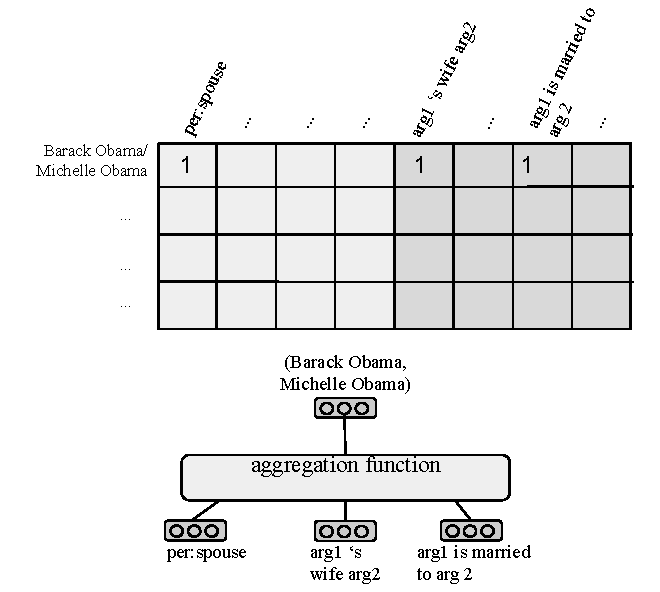
\includegraphics[scale=.68]{aggregate-entity}
\end{figure}


\subsection {Aggregation Functions}
In this work we examine several fairly simple aggregation functions.
\textbf{Mean Relation} creates a single centroid for the entity pair by averaging all of its relation vectors.
While this intuitive makes sense as an approximation for the explicit entity pair representation, averaging large numbers of embeddings can lead to a noisy signal.
The \textbf{Max Relation} represents the entity pair as its most similar relation to the query vector of interest.
This
 TopK Relations
 Dimension-wise Max Pool
   Convolution + Dimension-wise Max Pool


% results
\subsection{Results\label{sec:results}}


See Section~\ref{sec:details} for a discussion of the hyper-parameters, optimization techniques, etc. used in all experiments. As in~\citet{limin}, we train using the BPR loss of~\citet{rendle2009bpr}. 

%\begin{center}
%\begin{table}[h]
%\caption{english only models Results on english Tac.}
%\label{en-tac-table}
%\begin{tabular}{|l|l|l|l|}
%\hline
%\bf Model & \bf Recall & \bf Precision & \bf F1 \\
%\hline
%CNN & 28.86 & 35.89 & 31.99 \\
%CNN-parse & ?	 & ? & ? \\
%LSTM & 34.27 & 32.74 & 33.49  \\
%uschema:en & 29.40 & 42.60 & 34.79 \\
%uschema:en+LSTM+.1	    & ? & ? & ? \\
%uschema:en+LSTM+.1+alts	& ? & ? & ? \\
%\hline
%\end{tabular}
%\end{table}
%\end{center}


%\begin{center}
%\begin{table}[h]
%\caption{english + spanish models Results on english Tac. -D means dictionary, -N means no dictionary}
%\label{en-tac-table}
%\begin{tabular}{|l|l|l|l|}
%\hline
%\bf Model & \bf Recall & \bf Precision & \bf F1 \\
%\hline
%CNN-N & 28.86	 & 36.36	 & 32.17	 \\
%CNN-D & 29.75	 & 36.05	 & 32.59	 \\
%LSTM-N & 33.10 & 33.99 & 33.54 \\
%LSTM-D & 33.58 & 33.38 & 33.48 \\
%uschema:en-es & 29.68 & 44.78 & 35.70 \\
%uschema:en-es+LSTM-D+.1	        & 35.44 & 41.13 & 38.07 \\
%uschema:en-es+LSTM-D+.1+alts	& 37.49 & 42.14 & 39.68 \\
%\hline
%\end{tabular}
%\end{table}
%\end{center}



%% full english  + spanish results
%\begin{center}
%\begin{table}[h]
%\caption{ensemble results on english Tac. -D means dictionary, -N means no dictionary}
%\label{en-tac-ensemble-table}
%\begin{tabular}{|l|l|l|l|}
%\hline
%\bf Model & \bf Recall & \bf Precision & \bf F1 \\
%\hline
%%LSTM-D + .1 : & 22.48 & 42.99 & 29.52 \\
%%LSTM-D + .2 : & 13.64 & 52.93 & 21.69 \\
%uschema:en-es+LSTM-D	        & 39.75 & 33.03 & 36.08 \\
%uschema:en-es+LSTM-D+.1	        & 35.44 & 41.13 & 38.07 \\
%uschema:en-es+LSTM-D+.2	        & 32.08 & 44.40 & 37.25 \\
%uschema:en-es+LSTM-D+.1+alts	& 37.49 & 42.14 & 39.68 \\
%rel-factory                     & 35.02 & 46.97 & 40.13 \\
%rel-factory + LSTM-D+.1	        & 36.81 & 44.94 & 40.47 \\
%\hline
%\end{tabular}
%\end{table}
%\end{center}


%% full spanish results
%\subsection{Spanish Tac}
%\begin{center}
%\begin{table}[h]
%\caption{Results on spanish Tac}
%\label{es-tac-table}
%\begin{tabular}{|l|l|l|l|}
%\hline
%\bf Model & \bf Recall & \bf Precision & \bf F1 \\
%\hline
%CNN-N 		                    &  11.13       & 06.31        & 08.06   \\
%CNN-D 	                        &  12.78       & 11.21        & 11.95	\\
%LSTM-N 	                        &  07.37       & 09.80        & 08.41   \\
%LSTM-D  	                    &  10.38       & 28.87        & 15.27   \\
%%uschema    	                    &  26.17       & 14.37        & 18.55   \\
%%uschema +.1                     &  08.72       & 16.25        & 11.35   \\
%%uschema+.1+LSTM-D               &  15.64       & 18.94        & 17.13   \\
%uschema+.05                     &  20.90       & 17.64        & 19.13   \\
%uschema+.05+LSTM-N              &  ?       & ?        & ?   \\
%uschema+.05+LSTM-D              &  27.52       & 18.83        & 22.36   \\
%\hline
%\end{tabular}
%\end{table}
%\end{center}


\begin{table}[tb]
\begin{center}
\caption{Precision, recall and F1 of English-only models on the English TAC 2013 slot-filling task. LSTM+USchema ensemble outperforms any single model. \label{en-tac-table}}
\begin{tabular}{|lrrr|}
\hline
\bf Model & \bf Recall & \bf Precision & \bf F1 \\
\hline\hline
CNN                 & 28.9 & 35.9 & 32.0 \\
%CNN-parse           & ?	 & ? & ? \\
LSTM                & \bf 34.3 & 32.7 & 33.5  \\
USchema             & 29.4 & \bf 42.6 & 34.8 \\
\hline
USchema+LSTM        & 32.1 & 42.6 & 36.6 \\
USchema+LSTM+AN	& 34.4 & 43.9 & \bf 38.6 \\
\hline
\end{tabular}
\end{center}
\end{table}

\begin{table}[tb]
\begin{center}
\caption{F1 scores of multilingual models on the English TAC 2013 slot-filling task. Jointly embedding English and Spanish entity pairs results in higher scores on the English evaluation. \label{en-es-tac-table}}
\tabcolsep=0.15cm
\begin{tabular}{|lrrr|}
%\hspace{-10pt}
\hline
\bf Model & \bf En & \bf En+Es & \bf En+Es+dict  \\
\hline\hline
CNN  & 32.0 & 32.2 & 32.6	 \\
LSTM & 33.5 & 33.5 & 33.5 \\
USchema & 34.8 & 35.7  & --- \\
\hline
USchema+LSTM & 36.6 & 36.5 & 38.1 \\
USchema+LSTM+AN & 38.6 & 38.1  & \bf 39.7 \\
\hline
\end{tabular}
\end{center}

\end{table}

\begin{table}[h!]

\begin{center}
\caption{Zero-Annotation transfer learning F1 scores on 2012 Spanish TAC KBP slot-filling task. Adding a translation dictionary improves all encoder-based models. Ensembling LSTM and USchema models performs the best. \label{es-tac-table}}
\begin{tabular}{|lrr|}
\hline
\bf Model & \bf Es+En & \bf Es+En+dict  \\
\hline\hline
CNN 		                    & 8.1     & 12.0	\\
LSTM 	                        & 8.4     & 15.3   \\
USchema                         & 18.6     & --- \\
\hline
USchema+LSTM                    & 18.0     & \bf 22.4 \\
\hline
\end{tabular}
\end{center}
\end{table}



%In experiments on the English and Spanish TAC KBC slot-filling tasks, we find that both USchema and LSTM models outperform the CNN across languages, and that USchema tends to perform slightly better than the LSTM as the only model. Ensembling the LSTM and USchema models further increases final F1 scores in all experiments, suggesting that the two different types of model compliment each other well. In Section \ref{sec:qual-anal} we present a qualitative analysis of our results which further confirms this hypothesis.

Table \ref{en-tac-table} presents the performance of our English models. First, observe that the LSTM substantially outperforms a CNN. Second, note that the LSTM achieves higher recall than USchema whereas USchema is more precision-biased. This confirms our hypothesis in Section~\ref{sec:non-comp} about the strengths and weaknesses of the two approaches. 
%US, which matches more short, non-compositional patterns, makes more precise predictions at the cost of an inability to predict when entities are connected by a pattern unseen during training. The LSTM can predict a relation using any text between entities observes at test time, gaining recall at the loss of precision. 
Unsurprisingly, ensembling the LSTM and USchema improves F1 by nearly 2 points over the strongest single model, USchema. Adding the alternative names (AN) technique described in Section \ref{sec:ds-el} increases F1 by an additional 2 points, resulting in an F1 score that is competitive with the state-of-the-art.

In Table \ref{en-es-tac-table}, we analyze the effect of jointly learning English and Spanish models on English slot filling performance.  Adding Spanish data improves scores of USchema and CNN, though the LSTM remains unaffected. Further tying the parameters of English and Spanish data by adding a translation dictionary further improves the CNN, and greatly improves the ensemble of USchema and LSTM, leading to 1.5 point increase in F1 over the ensemble of models trained on English alone. The boost in score resulting from dictionary typing suggests that with dictionary-tied parameters the LSTM can better leverage the Spanish data to find good relations that USchema is unable to find with only parameter tying through entities. Since USchema embeds entire OpenIE patterns, and not single words, parameters cannot be tied at the word level and so dictionary-tied results are not applicable to this model. The final rows shows that the alternate names heuristic is complementary to improvements from including Spanish. 

Table \ref{es-tac-table} presents results for our Spanish relation extractors trained using zero-annotation transfer learning. For both the CNN and LSTM, tying word embeddings between the two languages results in substantial improvements. We see that ensembling the non-dictionary LSTM with USchema leads to a lower score than just USchema alone, but ensembling the dictionary-tied LSTM with USchema provides a significant increase of nearly 4 F1 points over the highest-scoring single model, USchema. Clearly, grounding the Spanish data using a translation dictionary provides much better Spanish word representations. These improvements are complementary to the baseline USchema model, and yield impressive results when ensembled. 


\subsection{Qualitative Analysis \label{sec:qual-anal}}

% error analysis
Analysis of our English models suggests that our encoder-based models (LSTM) extract relations based on a wide range of semantically similar patterns that the pattern-matching model (USchema) is unable to score due to a lack of exact string match in the test data. For example, Table \ref{tab:lstm-us-similar-rels} lists three examples of the \emph{per:children} relation that the LSTM finds which USchema does not, as well as three patterns that USchema does find. Though the LSTM patterns are all semantically and syntactically similar, they each contain different specific noun phrases, e.g. \emph{Lori}, \emph{four children}, \emph{toddler daughter}, \emph{Lee and Albert}, etc. Because these specific nouns weren't seen during training, USchema fails to find these patterns whereas the LSTM learns to ignore the specific nouns in favor of the overall pattern, that of a parent-child relationship in an obituary. USchema is limited to finding the relations represented by patterns observed during training, which limits the patterns matched at test-time to short and common patterns; all the USchema patterns matched at test time were similar to those listed in Table \ref{tab:lstm-us-similar-rels}: variants of \emph{'s son, '}. 


\begin{table}[h]
\begin{center}
\caption{Examples of the \emph{per:children} relation discovered by the LSTM and Universal Schema. Entities are bold and patterns italicized. The LSTM can model a richer set of patterns \label{tab:lstm-us-similar-rels}}
\small
\begin{tabular}{|p{8cm}|}
\hline
\multicolumn{1}{|c|}{\textbf{LSTM}} \\ \hline
{\bf McGregor} \emph{is survived by his wife, Lori, and four children, daughters Jordan,} { \bf Taylor} and Landri, and a son, Logan. \\ \hline
In addition to his wife, {\bf Mays} \emph{is survived by a toddler daughter and a son,} {\bf Billy Mays Jr.}, who is in his 20s. \\ \hline
{\bf Anderson} \emph{is survived by his wife Carol, sons Lee and Albert, daughter} {\bf Shirley Englebrecht} and nine grandchildren. \\
\hline\hline
\multicolumn{1}{|c|}{\textbf{USchema}}  \\ \hline
{\bf Dio} \emph{'s son,} {\bf Dan Padavona}, cautioned the memorial crowd to be screened regularly by a doctor and take care of themselves, something he said his father did not do. \\ \hline
But {\bf Marshall} \emph{'s son,} {\bf Philip}, told a different story.  \\ \hline
``I'd rather have Sully doing this than some stranger, or some hotshot trying to
be the next Billy Mays,'' said the guy who actually is the next {\bf Billy Mays}\emph{, his son} {\bf Billy Mays III}. \\ 
\hline
\end{tabular}
\end{center}
\end{table}

% cross lingual relations
Analysis of our multilingual models also suggests that they successfully embed semantically similar relations across languages using tied entity pairs and translation dictionary as grounding. Table \ref{tab:cross-lingual-relations} lists three top nearest neighbors in English for several Spanish patterns from the text. In each case, the English patterns capture the relation represented in the Spanish text. 

\newcommand{\tablespace}{\end{tabular}
\newline
\newline
%\hspace*{-21pt}
\begin{tabular}{|p{8cm}|}
}
\begin{table}[h]
\begin{center}
\caption{Top English patterns for a Spanish query pattern encoded using the dictionary LSTM: For each Spanish query (English translation in italics), a list of English nearest neighbors. \label{tab:cross-lingual-relations}}
\small
%\hspace*{-21pt}
\begin{tabular}{|p{8cm}|}
\hline
\argOne y cuatro de sus familias, incluidos su esposa, Wu Shu-chen, su hijo, \argTwo\\
\it{\argOne and four of his family members, including his wife, Wu Shu-chen, his son, \argTwo} \\
\hline
\argOne and his son \argTwo \\
\argOne is survived by his wife, Sybil MacKenzie and a son, \argTwo \\
\argOne gave birth to a baby last week -- son \argTwo \\
\hline
\tablespace
\hline
\argOne (Puff Daddy, cuyos verdaderos nombre sea \argTwo \\
\it{\argOne (Puff Daddy, whose real name is \argTwo} \\
\hline%\hline
\argOne (usually credited as {\it E1} \\
\argOne (also known as Gero \#\#, real name \argTwo \\
\argOne and (after changing his name to \argTwo \\
\hline
\tablespace
%\hline
%\argOne, Tian Tian, de \#\# a\~{n}os de edad, y su madre \argTwo\\
%\it{\argOne, Tian Tian, \#\# years old, and his mother \argTwo} \\
%\hline%\hline
%\argOne Gyllenhaal's parents -- screenwriter Naomi Foner and director \argTwo \\
%\argOne Brando's mother, actress Anna Kashfi, divorced \argTwo \\
%\argOne Cash, his mom was \argTwo \\
%\hline
%\tablespace
\hline
\argOne lleg\'{o} a la alfombra roja en compa\~{n}\'{i}a de su esposa, la actriz Suzy Amis, casi una hora antes que su ex esposa, \argTwo\\
\it{\argOne arrived on the red carpet with his wife, actress Suzy Amis, nearly an hour before his ex-wife , \argTwo} \\
\hline%\hline
\argOne, who may or may not be having twins with husband \argTwo \\
\argOne, aged twenty, Kirk married \argTwo\\
\argOne went to elaborate lengths to keep his wedding to former supermodel \argTwo\\
\hline
%\tablespace
%\hline
%\bf{{\it E1} , una firmes of estudios económicos lleven sede in {\it E2}}\\
%\it{{\it E1} an economic studies firm with headquarters in {\it E2}} \\
%\hline\hline
%{\it E2} offices of BP and {\it E1} \\
%{\it E2} , the Paris - based {\it E1} \\
%{\it E2} province , is the headquarters of {\it E1} \\
%\hline
\end{tabular}
\end{center}
\end{table}


In addition to embedding semantically similar phrases from English and Spanish to have high similarity, our models also learn high-quality multilingual word embeddings. In Table \ref{joint-word} we compare Spanish nearest neighbors of English query words learned by the LSTM with dictionary ties versus the LSTM with no ties, using no unsupervised pre-training for the embeddings. Both approaches jointly embed Spanish and English word types, using shared entity embeddings, but the dictionary-tied model learns qualitatively better multilingual embeddings. 


\begin{table}[h]
\setlength{\tabcolsep}{3pt}
\caption{Example English query words (not in translation dictionary) in bold with their top nearest neighbors by cosine similarity listed for the dictionary and no ties LSTM variants. Dictionary-tied nearest neighbors are consistently more relevant to the query word than untied. }
\label{joint-word}
\small
\begin{center}
%\begin{minipage}[b]{0.45\linewidth}
%\hspace*{-17pt}
\begin{tabular}{|ll|}
\hline
\multicolumn{2}{|c|}{ \bf CEO}\\
\multicolumn{1}{|c}{Dictionary} & \multicolumn{1}{c|} {No Ties} \\ \hline 
jefe (chief)    & CEO \\ 
CEO & director (principle) \\
ejecutivo (executive)   &  directora (director) \\
cofundador (cofounder)  & firma (firm) \\
president (chairman) & magnate (tycoon)\\
\hline
%
\multicolumn{2}{|c|}{\bf headquartered}\\
\multicolumn{1}{|c}{Dictionary} & \multicolumn{1}{c|} {No Ties} \\ \hline
sede (headquarters) & Geol\'{o}gico (Geological) \\
situado (located) & Treki (Treki) \\
selectivo (selective) & Geof\'{i}sico(geophysical) \\
profesional (vocational) & Normand\'{i}a (Normandy)\\
bas\'{a}ndose (based) & emplea (uses)\\
\hline
%\end{tabular}
%\end{minipage}
%\hspace{-12.5pt}
%\begin{minipage}[b]{0.45\linewidth}
%\begin{tabular}{|ll|}
%\hline
\multicolumn{2}{|c|}{\bf hubby}\\
\multicolumn{1}{|c}{Dictionary} & \multicolumn{1}{c|} {No Ties} \\ \hline 
matrimonio (marriage)  & esposa (wife) \\ 
casada (married) & esposo (husband) \\
esposa (wife) &  casada(married) \\
cas\'{o} (married) & embarazada (pregnant)  \\
embarazada (pregnant) & embarazo (pregnancy) \\
\hline

%
\multicolumn{2}{|c|}{\bf alias}\\
\multicolumn{1}{|c}{Dictionary} & \multicolumn{1}{c|} {No Ties} \\ \hline
simplificado (simplified) & Weaver (Weaver)\\ 
sabido (known) & interrogaci\'{o}n (question) \\
seud\'{o}nimo (pseudonym)  &  alias \\
privatizaci\'{o}n (privatisation)  & reelecto (reelected) \\
nombre (name)  & conocido (known)\\
\hline
\end{tabular}
%\end{minipage}
\end{center}
\end{table}






% conclusion
\section{Conclusion}
In this paper we explore the extension of Universal Schema that forgoes exlicit entity pair representations for an aggregatation function over mentions.
This extension allows us to handle all entity pairs - whether they were seen at train time or not - and also gives us a trivial connection to the provenance which made the prediction.
We present prelimanary findings for several aggregation functions including those that act on the individual relation level as well as those that learn to pool over groups of relations.
These prelimenary experiments were carried out on a fairly small dataset, we plan to test this on a much larger data set in the future.

In the future we plan two further extensions to this work.
The first is to improve the aggregation function with a query specific attention that will be able to proporitonally pool all evidence while simultaneously producing a weighting over provenanes.
The second extension will be to incorporate this work with existing work on Compositional Universal Schema creating a fully generalizable Universal Schema able to predict on all text.


\subsubsection*{Acknowledgments}

\bibliography{sources}
\bibliographystyle{naaclhlt2016}

\newpage
%\appendix
%\section{Appendix}

\subsection{Additional Qualitative Results}

Our model jointly embeds KB relations together with English and Spanish text. We demonstrate that plausible textual patterns are embedded close to the KB relations they express. Table \ref{tab:top-tac-patterns} shows top scoring English and Spanish patterns given sample relations from our TAC KB.

\begin{table}[h]
\begin{center}
%\hspace*{-20pt}
\begin{tabular}{|p{7.8cm}|}
\hline
\textbf{per:sibling} \\
\hline
   \argOne, seg\'{u}n petici\'{o}n the primeros ministro, \endgraf \hspace{5pt} su hermano gemelo \argTwo  			\\ %\cline{3-3}
  \argOne, sea the principal favorito para esto oficina \endgraf \hspace{5pt}que tambi\'{e}n ambiciona su hermano \argTwo 	\\%\cline{3-3}
  \argOne, y su hermano gemelo, the primeros ministro \argTwo 	\\
\hline
  \argOne, for whose brother \argTwo  		\\%\cline{3-3}
  \argOne inherited his brother \argTwo 	\\%\cline{3-3}
  \argOne on saxophone and brother \argTwo 	\\
\hline\hline
%
\textbf{org:top\_members\_employees} \\
\hline
   \argTwo, presidente y director generales the \argOne  			\\%\cline{3-3}
   	\argTwo, presidente of the negocios especializada \argOne  	\\%\cline{3-3}
   	\argTwo (CIA), the director of the entidad, \argOne 	\\
\hline
 \argTwo, vice president and policy director of the \argOne  		\\%\cline{3-3}
 \argTwo, president of the German Soccer \argOne 	\\%\cline{3-3}
  \argTwo, president of the quasi-official \argOne 	\\
\hline\hline
%%
\textbf{per:alternate\_names} \\
\hline
   \argOne(como tambi\'{e}n son sabido para \argTwo 			\\%\cline{3-3}
   \argTwo-cuyos verdaderos nombre sea \argOne 	\\%\cline{3-3}
   	\argOne  tambi\'{e}n sabido como \argTwo 	\\
\hline
   \argOne aka \argTwo 		\\%\cline{3-3}
   \argOne, who also creates music under the pseudonym \argTwo 	\\%\cline{3-3}
   \argOne( of Modern Talking fame ) aka \argTwo  	\\
\hline\hline
%%
\textbf{per:cities\_of\_residence} \\
 \hline
  \argOne, poblado d\'{o}nde vive \argTwo 			\\%\cline{3-3}
   \argOne, una ciudadano naturalizado american\endgraf \hspace{5pt} y nacido in \argTwo 	\\%\cline{3-3}
   \argOne, que vive in \argTwo 	\\
\hline
   \argOne was born Jan. \# , \#\#\#\# in \argTwo 		\\%\cline{3-3}
   	\argOne was born on Monday in \argTwo 	\\%\cline{3-3}
   \argOne was born at Keighley in \argTwo 	\\
\hline
\end{tabular}
\caption{Top scoring patterns for both Spanish (top) and English (bottom) given query TAC relations. \label{tab:top-tac-patterns}}
\end{center}
\end{table}

\subsection {Implementation and Hyperparameters}
\label{sec:details}
We performed a small grid search over learning rate {0.0001, 0.005, 0.001}, dropout {0.0, 0.01, 0.25, 0.5}, dimension {50, 100}, $\ell_2$ gradient clipping {1, 10, 50}, and epsilon {1e-8, 1e-6, 1e-4}. All models are trained for a maximum of 15 epochs. The CNN and LSTM both use 100d embeddings while USchema uses 50d. The CNN and LSTM both learned 100-dimensional word embeddings which were randomly initialized. Using pre-trained embeddings did not substantially affect the results. Entity pair embeddings for the baseline USchema model are randomly initialized. For the models with LSTM and CNN text encoders, entity pair embeddings are initialized using vectors from the baseline USchema model. This performs better than random initialization. We perform $\ell_2$ gradient clipping to 1 on all models. Universal Schema uses a batch size of 1024 while the CNN and LSTM use 128. All models are optimized using ADAM \citep{kingma2014adam} with $\epsilon=1e-8$, $\beta_1=0.9$, and $\beta_2=0.999$ with a learning rate of .001 for USchema and .0001 for CNN and LSTM. The CNN and LSTM also use dropout of 0.1 after the embedding layer.

\subsection{Details Concerning Cosine Similarity Computation}
\label{app:cosine}
We measure the similarity between $r_{\text{text}}$ and $r_{\text{schema}}$ by computing the vectors' cosine similarity. However, such a distance is not well-defined, since the model was trained using inner products between entity vectors and relation vectors, not between two relation vectors. The US likelihood is invariant to invertible transformations of the latent coordinate system, since $\sigma\left( u_{s,o}^\top v_r \right) = \sigma\left( (A^\top u_{s,o})^\top A^{-1} v_r \right)$ for any invertible $A$. When taking inner products between two $v$ terms, however, the implicit $A^{-1}$ terms do not cancel out. We found that this issue can be minimized, and high quality predictive accuracy can be achieved, simply by using sufficient $\ell_2$ regularization to avoid implicitly learning an $A$ that substantially stretches the space.

\subsection{Data Pre-processing, Distant Supervision and Extraction Pipeline \label{sec:ds-el}}

We replace tokens occurring less than 5 times in the corpus with UNK and normalize all digits to \# (e.g. Oct-11-1988 becomes Oct-\#\#-\#\#\#\#).
For each sentence, we then extract all entity pairs and the text between them as surface patterns, ignoring patterns longer than 15 tokens.
This results in 48 million English `relations'. In Section~\ref{sec:norm}, we describe a technique for normalizing the surface patterns.
We filter out entity pairs that occurred less than 10 times in the data and extract the largest connected component in this entity co-occurrence graph.
This is necessary for the baseline US model, as otherwise learning decouples into independent problems per connected component.
Though the components are connected when using sentence encoders, we use only a single component to facilitate a fair comparison between modeling approaches.
We add the distant supervision training facts from the RelationFactory system, i.e. 352,236 entity-pair-relation tuples obtained from Freebase and high precision seed patterns.
The final training data contains a set of 3,980,164 (KB and openIE) facts made up of 549,760 unique entity pairs, 1,285,258 unique relations and 62,841 unique tokens.

We perform the same preprocessing on the Spanish data, resulting in 34 million raw surface patterns between entities.
We then filter patterns that never occur with an entity pair found in the English data.  This yields 860,502 Spanish patterns.
Our multilingual model is trained on a combination of these Spanish patterns, the English surface patterns, and the distant supervision data described above.
We learn word embeddings for 39,912 unique Spanish word types.
After parameter tying for translation pairs (Section \ref{sec:tie-words}),  there are 33,711 additional Spanish words not tied to English.


\subsection{Generation of Cross-Lingual Tied Word Types}
\label{sec:word-tying}
We follow the same procedure for generating translation pairs as \cite{mikolov2013}. First, we select the top 6000 words occurring in the lowercased Europarl dataset for each language and obtain a Google translation. We then filter duplicates and translations resulting in multi-word phrases. We also remove English past participles (ending in -ed) as we found the Google translation interprets these as adjectives (e.g.,  `she read the borrowed book' rather than `she borrowed the book') and much of the relational structure in language we seek to model is captured by verbs. This resulted in 6201 translation pairs that occurred in our text corpus. Though higher quality translation dictionaries would likely improve this technique, our experimental results show that such automatically generated dictionaries perform well.


\subsection{Open IE Pattern Normalization}
\label{sec:norm}
To improve US generalization, our US relations use log-shortened patterns where the middle tokens in patterns longer than five tokens are simplified. For each long pattern we take the first two tokens and last two tokens, and replace all $k$ remaining tokens with the number $\log k$. For example, the pattern {\bf Barack Obama} {\it is married to a person named} {\bf Michelle Obama} would be converted to: {\bf Barack Obama} {\it is married [1] person named} {\bf Michell Obama}. This shortening performs slightly better than whole patterns. LSTM and CNN variants use the entire sequence of tokens.





\end{document}
